%% FullCourse_10Lecs -- Lecture 1, Topic 1.3a: Model Extensions and Challenges
%% Source: ./archive_pre_split/Lec01_Quant_Macro.tex (section 5)
%% Pass A mechanical split (verbatim content preserved).
%% Sub-split: T3 was split into T3a (§5) and T3b (§6) because §5+§6 = 32 frames > 30-slide ceiling.

%% Shared preamble for the FullCourse_10Lecs topic decks.
%%
%% Each topic .tex \input's this file, then defines its own \title, \date
%% override (if any), \graphicspath, and \begin{document}.
%%
%% Reconstructed verbatim from the inlined copy preserved in
%% Lec10_Case_Studies/Lec10_T8_Case6_DeepRamsey.tex (lines 23-190), which is
%% explicitly annotated there as "from ../shared_preamble.tex, copied verbatim".
%% Base preamble matches MiniCourse_8hr/Slides/shared_preamble.tex; this version
%% additionally provides \sectiondivider, the conceptbox/cautionbox/examplebox/
%% takeawaybox tcolorboxes, and \compacttables used across the split decks.

\documentclass[10pt,english,aspectratio=169]{beamer}

\usepackage{ae,aecompl}
\usepackage[T1]{fontenc}
\usepackage{textcomp}
\usepackage[utf8]{inputenc}
\usepackage{babel}
\usepackage{datetime2}

\setcounter{secnumdepth}{3}
\setcounter{tocdepth}{3}

\usepackage{amsmath, amssymb, amsthm, graphicx}
\usepackage{booktabs, multirow}
\usepackage{tikz}
\usepackage{pgfplots}
\pgfplotsset{compat=1.16}
\usepackage[most]{tcolorbox}
\tcbuselibrary{skins, breakable, theorems}
\usepackage{listings}
\usepackage{xcolor}

\lstset{
  basicstyle=\ttfamily\small,
  keywordstyle=\color{blue!80!black}\bfseries,
  commentstyle=\color{green!50!black}\itshape,
  stringstyle=\color{orange!80!black},
  backgroundcolor=\color{gray!8},
  frame=single,
  rulecolor=\color{gray!40},
  breaklines=true,
  showstringspaces=false,
  numbers=none,
}

\lstdefinestyle{pythonstyle}{
    language=Python,
    basicstyle=\ttfamily\footnotesize,
    keywordstyle=\color{blue!80!black}\bfseries,
    commentstyle=\color{green!50!black}\itshape,
    stringstyle=\color{orange!80!black},
    frame=single,
    breaklines=true,
    showstringspaces=false,
    numbers=left,
    numbersep=5pt,
    numberstyle=\tiny\color{gray},
    backgroundcolor=\color{gray!8},
    rulecolor=\color{gray!40}
}

\ifx\hypersetup\undefined
  \AtBeginDocument{%
    \hypersetup{bookmarks=false,breaklinks=true,pdfborder={0 0 0},colorlinks=true,
      linkcolor=DarkText,urlcolor=RedTitle}%
  }
\else
  \hypersetup{bookmarks=false,breaklinks=true,pdfborder={0 0 0},colorlinks=true,
    linkcolor=DarkText,urlcolor=RedTitle}%
\fi

\makeatletter
\newcommand\makebeamertitle{%
  \begin{frame}[plain]
    \vspace*{1.0cm}
    \centering
    {\usebeamerfont{title}\usebeamercolor[fg]{title}\inserttitle\par}
    \vspace{1.0cm}
    {\usebeamerfont{author}\usebeamercolor[fg]{author}\insertauthor\par}
    \vspace{0.2cm}
    {\usebeamerfont{date}\usebeamercolor[fg]{date}\insertdate\par}
  \end{frame}}%
\AtBeginDocument{%
  \let\origtableofcontents=\tableofcontents
  \def\tableofcontents{\@ifnextchar[{\origtableofcontents}{\gobbletableofcontents}}
  \def\gobbletableofcontents#1{\origtableofcontents}%
}

\usetheme{metropolis}
\usefonttheme{professionalfonts}

\definecolor{LightGray}{RGB}{230,230,230}
\definecolor{RedTitle}{RGB}{0,0,200}
\definecolor{VeryLightGray}{RGB}{245,245,245}
\definecolor{DarkText}{RGB}{0,0,0}

\setbeamercolor{background canvas}{bg=white}
\setbeamercolor{title}{fg=RedTitle}
\setbeamercolor{author}{fg=DarkText}
\setbeamercolor{date}{fg=DarkText}
\setbeamercolor{frametitle}{bg=VeryLightGray,fg=DarkText}
\setbeamercolor{normal text}{fg=DarkText}
\setbeamerfont{title}{size=\large}

\setbeamersize{text margin left=5mm, text margin right=5mm}
\addtobeamertemplate{frametitle}{}{\vspace{-0.5em}}
\newcommand{\reducevspace}{\vspace{-0.5cm}}

% Shared section divider and box styles for split topic decks.
\newcommand{\sectiondivider}[2]{%
\begin{frame}[plain,noframenumbering]
\begin{center}
\vfill
{\Large\textbf{#1}\par}
\vspace{0.35cm}
{\normalsize #2\par}
\vfill
\end{center}
\end{frame}
}

\newtcolorbox{conceptbox}[1][]{
  colback=blue!3,
  colframe=RedTitle!55,
  boxrule=0.35mm,
  arc=1mm,
  left=2mm,
  right=2mm,
  top=1mm,
  bottom=1mm,
  #1
}
\newtcolorbox{cautionbox}[1][]{
  colback=red!3,
  colframe=red!50!black,
  boxrule=0.35mm,
  arc=1mm,
  left=2mm,
  right=2mm,
  top=1mm,
  bottom=1mm,
  #1
}
\newtcolorbox{examplebox}[1][]{
  colback=green!3,
  colframe=green!45!black,
  boxrule=0.35mm,
  arc=1mm,
  left=2mm,
  right=2mm,
  top=1mm,
  bottom=1mm,
  #1
}
\newtcolorbox{takeawaybox}[1][]{
  colback=VeryLightGray,
  colframe=RedTitle!55,
  boxrule=0.35mm,
  arc=1mm,
  left=2mm,
  right=2mm,
  top=1mm,
  bottom=1mm,
  #1
}
\newcommand{\compacttables}{\renewcommand{\arraystretch}{1.15}}

\setbeamertemplate{navigation symbols}{}
\setbeamertemplate{footline}{%
  \hfill%
  \usebeamercolor[fg]{page number in head/foot}%
  \usebeamerfont{page number in head/foot}%
  \insertframenumber\,/\,\inserttotalframenumber\kern1em\vskip2pt%
}

\makeatother

\author{Zhigang Feng}
% "date with time": compile timestamp so each build is identifiable.
\date{\today\ \DTMcurrenttime}


\graphicspath{{./pic/}{../../FullCourse_10Lecs/Lec01_Quant_Macro/pic/}{../}}

\title[AI for Econ Research]{AI for Economic Research: Dynamic Models, Language, and Agents\\
Lecture 1.3a: Model Extensions and Theoretical Challenges}

\begin{document}

\makebeamertitle

%=============================================================================
\begin{frame}{Topic 1.3a Agenda}
\begin{enumerate}
  \item \textbf{Heterogeneous Agent Models} --- Aiyagari, Krusell--Smith
  \medskip
  \item \textbf{Theoretical Issues} --- existence, uniqueness, continuity
  \medskip
  \item \textbf{Curse of Dimensionality} --- the computational wall
  \medskip
  \item \textbf{Numerical Methods} --- interpolation, optimization, simulation
  \medskip
  \item \textbf{Calibration, Estimation, Accuracy} --- mapping models to data
  \medskip
  \item \textbf{Perturbation Methods} --- and supplementary video resource
\end{enumerate}
\end{frame}

%=============================================================================
\section{Model Extensions and Challenges}

\begin{frame}{Extensions Based on the Optimal Growth Model}
\begin{center}
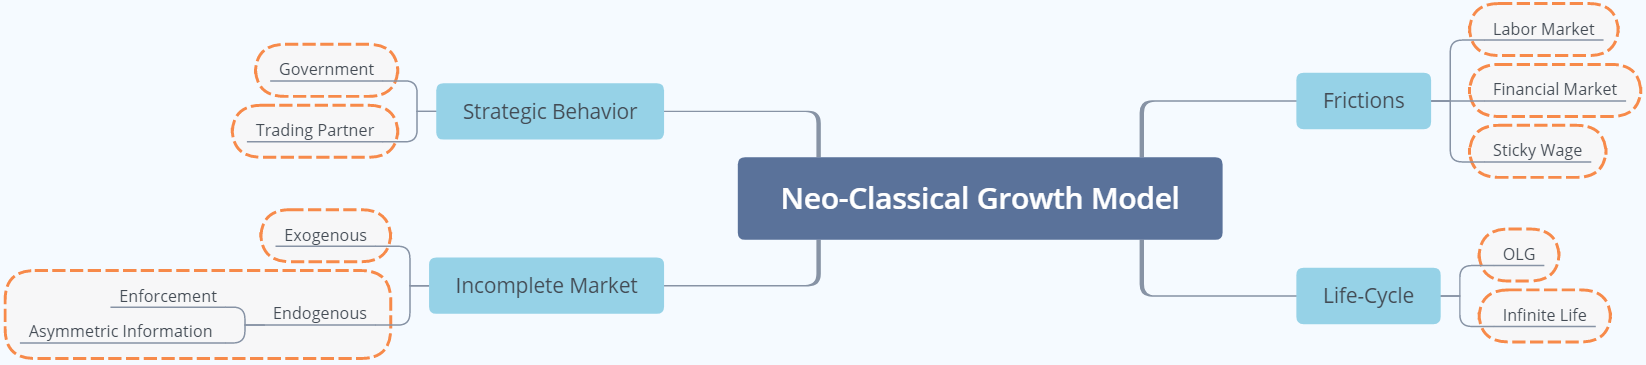
\includegraphics[width=12cm,height=8cm]{pic/neoclastruct}
\par\end{center}
\end{frame}

\begin{frame}{Heterogeneous Agents: Breaking the Simplicity}
\begin{itemize}
\item \textbf{Realistic Extension:} Agents differ in wealth, income, productivity
\begin{itemize}
    \item Individual state: $(a_i, z_i)$ --- assets and idiosyncratic shock
    \item Now $k_i \neq K$; individual choices don't reveal aggregates
\end{itemize}

\medskip
\item \textbf{Prices Depend on the Distribution:}
\[
r = r(\mu), \qquad w = w(\mu)
\]
where $\mu$ is the \emph{cross-sectional distribution} of $(a, z)$

\medskip
\item \textbf{The Distribution Is a State Variable:}
\begin{itemize}
    \item To forecast prices, agents must forecast how $\mu$ evolves
    \item But $\mu$ is \emph{infinite-dimensional}---a measure over $(a, z)$
    \item Evolution: $\mu' = \Phi(\mu; g)$ depends on everyone's policy
\end{itemize}

\medskip
\item \textbf{The Environment Is No Longer Obvious:}
\begin{itemize}
    \item Agents face a \emph{perceived law of motion} they must approximate
    \item First Welfare Theorem fails $\Rightarrow$ must solve for prices explicitly
\end{itemize}
\end{itemize}
\end{frame}

\begin{frame}{Bewley-Aiyagari-Huggett Model}
\begin{itemize}
\item \textbf{Setup:}
\begin{itemize}
    \item Continuum of infinitely lived households (measure 1)
    \item Uninsurable idiosyncratic income shocks $\epsilon$
    \item \emph{Ex-ante} identical, \emph{ex-post} heterogeneous
\end{itemize}

\medskip
\item \textbf{Bellman Equation:}
\[
v(a,\epsilon;\lambda)=\max_{c,a'}\left\{ u(c)+\beta\sum_{\epsilon'}v(a',\epsilon';\lambda')\pi(\epsilon,\epsilon') \right\}
\]
subject to:
\begin{align*}
c+a' & = (1+r(\lambda))a+w(\lambda)\epsilon \\
a' & \geq -\underline{a}
\end{align*}

\medskip
\item \textbf{Stationary Equilibrium:} Find $\lambda^*$ such that $\lambda^* = \Phi(\lambda^*; g)$
\begin{itemize}
    \item Distribution is invariant under optimal policies
    \item Incomplete markets endogenously generate wealth inequality
\end{itemize}
\end{itemize}
\end{frame}

\begin{frame}{Krusell-Smith Model}
\begin{itemize}
\item \textbf{Extension:} Add \emph{aggregate uncertainty} to Aiyagari

\medskip
\item \textbf{Aggregate shock:} $z_t \in \{z_g, z_b\}$ (good/bad states)
\begin{itemize}
    \item Affects aggregate productivity
    \item Unemployment higher in bad states: $u_b > u_g$
\end{itemize}

\medskip
\item \textbf{Household Problem:}
\[
v(k,\epsilon;\Gamma,z)=\max_{c,k'} \left\{ U(c)+\beta \, \mathbb{E}[v(k',\epsilon';\Gamma',z') \mid z,\epsilon] \right\}
\]
subject to:
\begin{align*}
c+k' &= r(\bar{k},\bar{l})k + w(\bar{k},\bar{l})\epsilon + (1-\delta)k \\
\Gamma' &= H(\Gamma,z,z'), \qquad k' \geq 0
\end{align*}

\medskip
\item \textbf{The Challenge:} Agents must forecast evolution of $\Gamma$---infinite-dimensional!
\end{itemize}
\end{frame}

\begin{frame}{Krusell-Smith: The Computational Innovation}
\begin{itemize}
\item \textbf{Key Insight (Krusell-Smith, 1998):}
\begin{itemize}
    \item Agents don't need to track the entire distribution $\Gamma$
    \item Approximate with low-dimensional moments: $\bar{K} = \int k \, d\Gamma$
\end{itemize}

\medskip
\item \textbf{Bounded Rationality:} Agents use simple forecasting rules
\[
\log \bar{K}' = a_0(z) + a_1(z) \log \bar{K}
\]

\medskip
\item \textbf{Algorithm:}
\begin{enumerate}
    \item Guess coefficients $(a_0, a_1)$
    \item Solve individual problem given forecasting rule
    \item Simulate economy, regress $\log \bar{K}'$ on $\log \bar{K}$
    \item Update coefficients; iterate until convergence
\end{enumerate}

\medskip
\item \textbf{Remarkable Finding:} $R^2 > 0.999$---mean capital is nearly sufficient!
\end{itemize}
\end{frame}

\begin{frame}{Theoretical Issues in Heterogeneous Agent Models}
\begin{itemize}
\item \textbf{Existence of Recursive Equilibrium:}
\begin{itemize}
    \item When markets are complete/efficient: easier to prove
    \item Incomplete markets: may require forward-looking variables
\end{itemize}

\medskip
\item \textbf{Uniqueness:} Generally \emph{not} guaranteed
\begin{itemize}
    \item Multiple steady states possible
    \item Policy functions may have discontinuities
\end{itemize}

\medskip
\item \textbf{Continuity:} Value and policy functions may not be continuous in aggregates

\medskip
\item \textbf{Computation:}
\begin{itemize}
    \item Curse of dimensionality (distribution as state)
    \item Ensuring accuracy of approximations
    \item Verifying equilibrium conditions
\end{itemize}

\medskip
\item \textbf{These issues become more severe in optimal policy (Ramsey) problems.}
\end{itemize}
\end{frame}

\begin{frame}{Example: Non-Existence of Continuous Equilibrium}
\textbf{Santos (2002):} Representative household, $\sum \beta^t \log(c_t)$, subject to:
\[
c_{t}+k_{t+1} \leq \pi_{t}+(1-\tau_{t})r_{t}k_{t}+T_{t}
\]
with piecewise linear tax on capital:
\[
\tau(K) = \begin{cases}
0.10 & \text{if } K \leq 0.160 \\
0.05 - 10(K - 0.165) & \text{if } 0.160 < K < 0.170 \\
0 & \text{if } K \geq 0.170
\end{cases}
\]

\medskip
\textbf{Result:} A continuous Markov equilibrium \emph{fails to exist}.
\begin{itemize}
    \item Middle steady state: unstable (complex eigenvalues)
    \item Other steady states: saddle-path stable
    \item Equilibrium exhibits cycles or discontinuities
\end{itemize}
\end{frame}

\begin{frame}{Theoretical Issues: Equilibrium Cycles}
\begin{center}
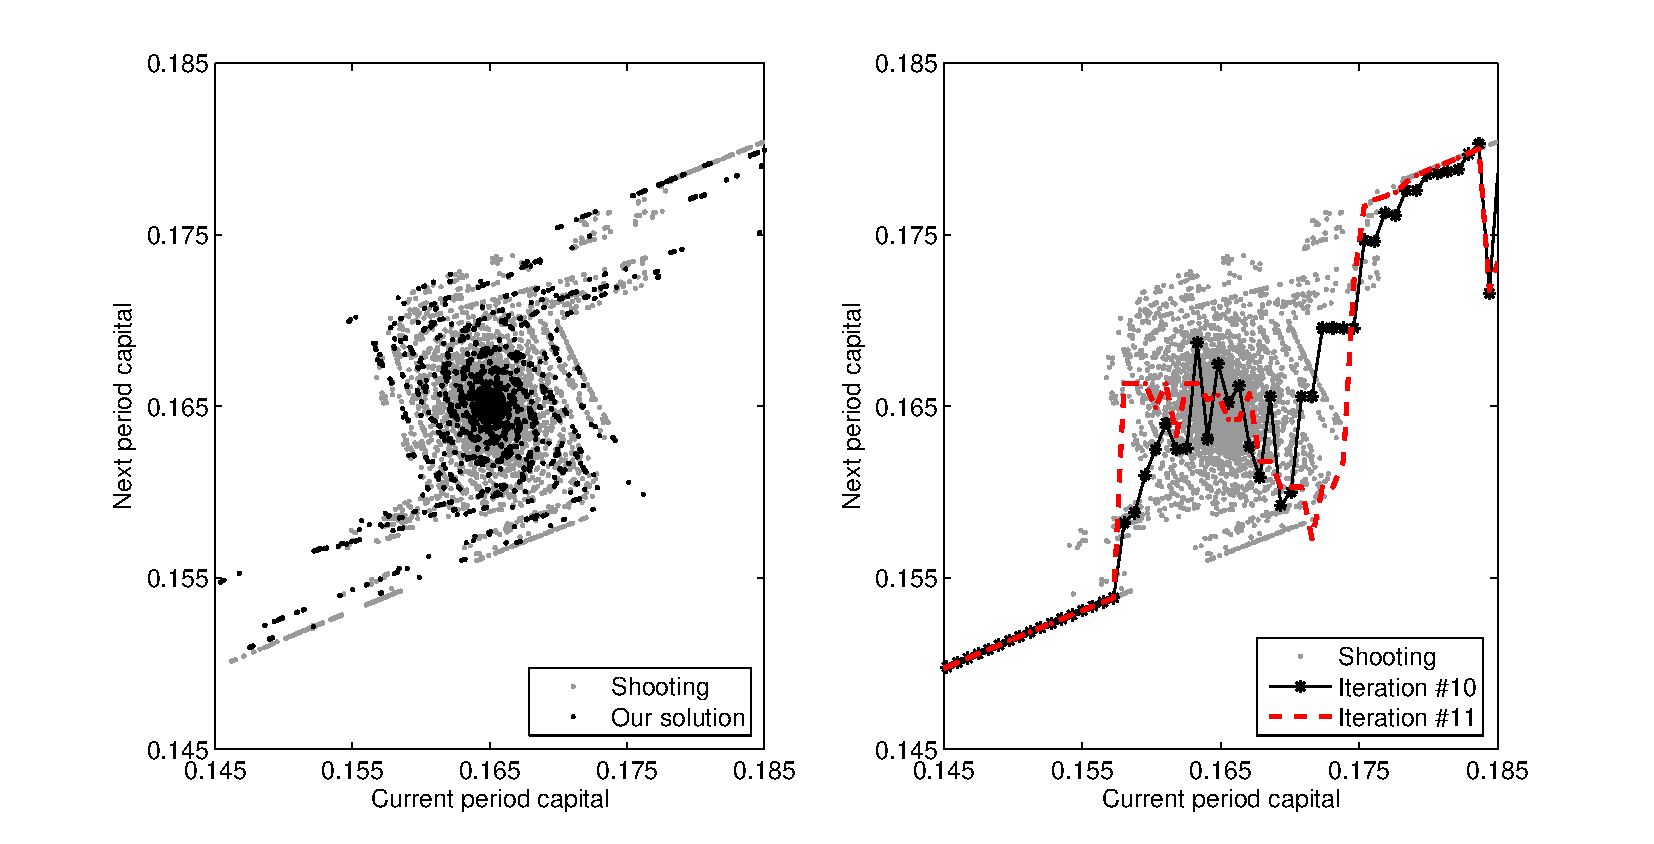
\includegraphics[width=11cm,height=7cm]{pic/cycle_compare}
\par\end{center}
\end{frame}

\begin{frame}{Ramsey Problem: Additional State Variables}
\begin{itemize}
\item \textbf{Consumer FOCs:}
\begin{itemize}
    \item Consumption: $\lambda_{t}=u_{c_t}$
    \item Labor: $u_{n}=(1-\tau_{t})u_{c}f_{n}$
    \item Euler: $\lambda_{t}=\lambda_{t+1}\beta[(1-\theta_{t+1})f_{k}+1-\delta]$
\end{itemize}

\medskip
\item \textbf{The Problem:} Euler equation can be rewritten backward:
\[
\lambda_{t-1}=\lambda_{t}\beta[(1-\theta_{t})f_{k}(k_{t},n_{t})+1-\delta]
\]

\medskip
\item \textbf{Implication:} Must track $\lambda_{t-1}$ as a state variable
\begin{itemize}
    \item Minimal state space $(k_t)$ is \emph{insufficient}
    \item Need $(k_t, \lambda_{t-1})$ with unknown domain for $\lambda$
\end{itemize}

\medskip
\item \textbf{Consequence:} State space expands; recursive formulation becomes more complex.
\end{itemize}
\end{frame}

\begin{frame}{The Curse of Dimensionality}
\begin{itemize}
\item \textbf{Bellman (1957):} Named the ``curse of dimensionality''---exponential growth of computational cost with state dimension.

\medskip
\item \textbf{Grid-Based Methods:}
\begin{itemize}
    \item $n$ grid points per dimension, $d$ dimensions $\Rightarrow$ $n^d$ total points
    \item Example: 100 points $\times$ 10 dimensions = $10^{20}$ points
    \item Infeasible for storage, let alone computation
\end{itemize}

\medskip
\item \textbf{Heterogeneous Agent Models:}
\begin{itemize}
    \item Distribution $\mu$ is infinite-dimensional
    \item Even discretized: thousands of $(a, z)$ pairs $\times$ aggregate states
    \item Standard VFI becomes computationally prohibitive
\end{itemize}

\medskip
\item \textbf{This is exactly the challenge AI/RL research confronts}---in even more extreme settings.
\end{itemize}
\end{frame}

\begin{frame}{Numerical Methods: Interpolation and Approximation}
\begin{itemize}
\item \textbf{Purpose:} Represent value and policy functions on a computer.

\medskip
\item \textbf{Interpolation Methods:}
\begin{itemize}
    \item \emph{Linear interpolation:} Simple, fast, not smooth
    \item \emph{Cubic splines:} Smooth, accurate for smooth functions
    \item \emph{Chebyshev polynomials:} Near-optimal approximation on $[-1,1]$; avoid Runge's phenomenon
\end{itemize}

\medskip
\item \textbf{Discretization of Stochastic Processes:}
\begin{itemize}
    \item \emph{Tauchen (1986):} Discretize AR(1) $z_t = \rho z_{t-1} + \sigma \varepsilon_t$ via finite Markov chain
    \item \emph{Rouwenhorst (1995):} Better for highly persistent processes ($\rho \approx 1$)
\end{itemize}

\medskip
\item \textbf{Projection Methods:}
\begin{itemize}
    \item Approximate $v(k) \approx \sum_j c_j \phi_j(k)$ using basis functions
    \item Choose coefficients to minimize residuals in Bellman equation
\end{itemize}
\end{itemize}
\end{frame}

\begin{frame}{Numerical Methods: Optimization}
\begin{itemize}
\item \textbf{Maximization in the Bellman Equation:}
\[
\max_{k' \in \Gamma(k)} \left\{ u(f(k) - k') + \beta v(k') \right\}
\]

\medskip
\item \textbf{Classical Methods:}
\begin{itemize}
    \item \emph{Grid search:} Evaluate objective at all grid points; pick max --- reliable but slow
    \item \emph{Golden section search:} Exploit unimodality; $O(\log n)$ evaluations
    \item \emph{Newton-Raphson:} Use derivatives for fast convergence; $O(\text{quadratic})$
\end{itemize}

\medskip
\item \textbf{Modern Methods:}
\begin{itemize}
    \item \emph{Automatic differentiation (PyTorch):} Exact gradients from code
    \item \emph{Stochastic gradient descent (SGD/Adam):} Scale to high dimensions
    \item \emph{Gradient-based optimization:} Essential for neural network training
\end{itemize}

\medskip
\item \textbf{Rule of Thumb:} Use derivatives when available; they dramatically speed up convergence.
\end{itemize}
\end{frame}

\begin{frame}{Numerical Methods: Simulation}
\begin{itemize}
\item \textbf{Monte Carlo Simulation:} Generate artificial time series from a calibrated model.

\medskip
\item \textbf{Algorithm:}
\begin{enumerate}
    \item Draw shocks $\{z_t\}_{t=1}^T$ from the Markov chain
    \item Given policy $g$, compute $k_{t+1} = g(k_t, z_t)$ and $c_t = f(k_t, z_t) - k_{t+1}$
    \item Compute moments: mean, variance, autocorrelation, cross-correlations
\end{enumerate}

\medskip
\item \textbf{Uses in Quantitative Macro:}
\begin{itemize}
    \item \emph{Calibration:} Match model moments to data moments
    \item \emph{Counterfactuals:} Study effects of policy changes
    \item \emph{Distribution computation:} Simulate agent distribution in HA models
\end{itemize}

\medskip
\item \textbf{Key Consideration:} Burn-in period; law of large numbers requires $T \to \infty$
\end{itemize}
\end{frame}

\begin{frame}{Calibration: Mapping Models to Data}
\begin{itemize}
\item \textbf{Goal:} Choose model parameters $\theta = (\beta, \alpha, \delta, \sigma, \rho, \ldots)$ so the model matches key empirical regularities.

\medskip
\item \textbf{Calibration Strategies:}
\begin{enumerate}
    \item \emph{Direct calibration:} Match parameter to single data moment directly\\
        \quad e.g., $\alpha = $ labor share $\approx 0.36$; $\delta = $ depreciation rate $\approx 0.10$
    \item \emph{Indirect calibration:} Choose $\theta$ to minimize distance between model and data moments\\
        \quad e.g., $\beta$ calibrated to match capital-output ratio
    \item \emph{Steady-state calibration:} Use steady-state conditions as moment restrictions
\end{enumerate}

\medskip
\item \textbf{Typical Moments Targeted:}
\begin{itemize}
    \item Capital-output ratio, consumption-output ratio
    \item Labor share, average hours worked
    \item Volatility and autocorrelation of GDP, consumption, investment
    \item Cross-sectional wealth and income inequality
\end{itemize}
\end{itemize}
\end{frame}

\begin{frame}{Estimation: Formal Inference}
\begin{itemize}
\item \textbf{Calibration vs.\ Estimation:}
\begin{itemize}
    \item Calibration: informal, one-to-one moment matching
    \item Estimation: formal statistical framework, uncertainty quantification
\end{itemize}

\medskip
\item \textbf{Simulated Method of Moments (SMM):}
\[
\hat{\theta} = \arg\min_\theta \left[ m_{\text{data}} - m_{\text{model}}(\theta) \right]' W \left[ m_{\text{data}} - m_{\text{model}}(\theta) \right]
\]
where $W$ is a weighting matrix; accounts for estimation uncertainty.

\medskip
\item \textbf{Indirect Inference (Gourieroux et al., 1993):}
\begin{itemize}
    \item Fit auxiliary model to both data and simulated data
    \item Match the \emph{auxiliary model parameters}
    \item Useful when data has complex time-series structure
\end{itemize}

\medskip
\item \textbf{Bayesian Methods:}
\begin{itemize}
    \item Prior $p(\theta)$ + likelihood $p(\text{data}|\theta)$ $\Rightarrow$ posterior $p(\theta|\text{data})$
    \item MCMC sampling; popular for DSGE models
\end{itemize}
\end{itemize}
\end{frame}

\begin{frame}{Accuracy Analysis: How Good Is the Solution?}
\begin{itemize}
\item \textbf{Problem:} Numerical methods produce approximations. How do we measure quality?

\medskip
\item \textbf{Euler Equation Residuals (Judd, 1992):}
\[
\text{EEE}(k) = \left| 1 - \frac{\beta u'(c_{t+1}) F_k(k_{t+1}, z_{t+1})}{u'(c_t)} \right|
\]
\begin{itemize}
    \item Measures how well the computed policy satisfies optimality conditions
    \item Interpretation: fraction of consumption (``dollar unit'') wasted by approximation error
    \item Target: $|\text{EEE}| < 10^{-4}$ (less than 0.01\% error)
\end{itemize}

\medskip
\item \textbf{Den Haan-Marcet Test:} Statistical test for whether forecast errors are unpredictable --- checks if optimality conditions hold on average.

\medskip
\item \textbf{Policy Function Comparison:} Compare solution across methods (VFI, EGM, projection) to verify agreement.
\end{itemize}
\end{frame}

\begin{frame}{Perturbation Methods: Linearization}
\begin{itemize}
\item \textbf{Idea:} Approximate the equilibrium around the deterministic steady state.

\medskip
\item \textbf{First-Order Perturbation (Log-linearization):}
\[
\hat{x}_{t+1} \approx A \hat{x}_t + B \hat{z}_t
\]
where $\hat{x}_t = \log x_t - \log x^*$ are log-deviations from steady state.
\begin{itemize}
    \item Fast and tractable; the workhorse of DSGE estimation (Dynare)
    \item Ignores risk---agents behave as if the future is certain
\end{itemize}

\medskip
\item \textbf{Higher-Order Perturbation:}
\begin{itemize}
    \item 2nd order: captures precautionary saving, risk premia
    \item 3rd order: skewness, asymmetric responses to shocks
    \item Dramatically more complex, but still closed-form
\end{itemize}

\medskip
\item \textbf{Limitation:} Valid only near steady state; fails for large shocks or crises.
\end{itemize}
\end{frame}

\begin{frame}{Supplementary Resource: Classical Numerical Methods}
\begin{tcolorbox}[colback=blue!3, colframe=blue!40, title=Video Lecture Series]
Complete recordings of classical computational methods for macroeconomists are available at:
\begin{center}
\url{https://space.bilibili.com/2142649036/lists/7180709}
\end{center}
\medskip
Topics include:
\begin{itemize}
  \item Numerical solution methods: value function iteration, time iteration
  \item Advanced methods: Howard improvement, endogenous grid method (EGM)
  \item Perturbation methods (first- and second-order)
  \item Projection methods: Chebyshev polynomials, collocation
  \item Numerical optimization, interpolation, and simulation
  \item High-performance and parallel computing (MPI, GPU)
\end{itemize}
\end{tcolorbox}
\end{frame}

\end{document}
